% 有限差分法求解电位基本方程 - 实验报告
\documentclass{../ElectromagneticFieldTemplate}

\graphicspath{{./Figures/}{../TemplateFigures/}}

\setExperimentInfo
    {有限差分法求解电位基本方程}
    {2024217802}
    {严子竣}
    {2024212622}
    {张璇}
    {\today}

\begin{document}

\maketitle

\section{实验目的}

\begin{enumerate}
    \item 理解有限差分法的基本原理，通过本实验能够理解有限差分法的基本概念，特别是如何用差商代替微商来近似求解微分方程。
    \item 掌握有限差分法在直角坐标系中的应用，能够在直角坐标系中应用有限差分法求解电位的基本方程（泊松方程、拉普拉斯方程）。
    \item 能够使用 Matlab 结合 DeepSeek 编写有限差分法的求解程序，分析结果，并通过调整参数观察其对结果的影响。
    \item 能够根据实验结果撰写详细的实验报告，包括实验目的、原理、步骤、结果图和个人的思考与分析。
\end{enumerate}

\section{实验原理与说明}

\subsection{有限差分法基本原理}
有限差分法（Finite Difference Method, FDM）是一种数值求解偏微分方程的重要方法。其核心思想是利用差分公式近似代替导数（微商），将连续区域离散化为网格节点，将微分方程转化为代数方程组。

对于二维静电场，电位 \(\phi(x,y)\) 满足泊松方程：
\[
\frac{\partial^2 \phi}{\partial x^2} + \frac{\partial^2 \phi}{\partial y^2} = -\frac{\rho}{\varepsilon_0}
\]
当 \(\rho=0\) 时退化为拉普拉斯方程。

在均匀网格（\(\Delta x = \Delta y = h\)）下，二阶偏导数的中心差分近似为：
\[
\frac{\partial^2 \phi}{\partial x^2} \approx \frac{\phi_{i+1,j} - 2\phi_{i,j} + \phi_{i-1,j}}{h^2}, \quad
\frac{\partial^2 \phi}{\partial y^2} \approx \frac{\phi_{i,j+1} - 2\phi_{i,j} + \phi_{i,j-1}}{h^2}
\]
代入泊松方程并整理，得到内部节点的迭代公式：
\[
\phi_{i,j} = \frac{1}{4}\left( \phi_{i+1,j} + \phi_{i-1,j} + \phi_{i,j+1} + \phi_{i,j-1} + h^2 \frac{\rho}{\varepsilon_0} \right)
\]

\subsection{超松弛迭代法（SOR）}
为了加速收敛，采用超松弛迭代法（Successive Over-Relaxation, SOR）：
\[
\phi_{i,j}^{(k+1)} = (1-\omega)\phi_{i,j}^{(k)} + \omega \phi_{i,j}^{(k+1,\text{GS})}
\]
其中 \(\phi_{i,j}^{(k+1,\text{GS})}\) 为高斯-赛德尔迭代值，\(\omega \in (1,2)\) 为松弛因子。本实验取 \(\omega=1.8\)，收敛容差 \(10^{-6}\)。

\section{实验设备}

\begin{itemize}
    \item 软件：Matlab R2023a、DeepSeek AI 辅助编程
    \item 硬件：个人计算机
\end{itemize}

\section{实验内容}

通过有限差分法求解直角坐标系中 \(1\,\text{m}\times 1\,\text{m}\) 正方形区域的电位边值问题，分别设置四种不同的边界条件或电荷分布，观察并分析电位分布的变化：

\begin{enumerate}
    \item \textbf{拉普拉斯方程，上边界为 1 V，其余边界接地（0 V）}；
    \item \textbf{拉普拉斯方程，上边界 0.5 V，右边界 1 V，其余边界 0 V}；
    \item \textbf{拉普拉斯方程，上下边界分别为 1 V 和 -1 V，左右边界呈线性插值}；
    \item \textbf{泊松方程，四边接地，内部均匀体电荷密度 \(\rho=10^{-6}\,\text{C/m}^3\)}。
\end{enumerate}

\section{实验步骤}

\begin{enumerate}
    \item \textbf{理论学习}：阅读相关资料，理解有限差分法及其在直角坐标系中求解电位的原理。
    \item \textbf{问题定义}：确定求解区域 \(x\in[0,1], y\in[0,1]\)，网格大小 \(51\times 51\)（\(\Delta x=\Delta y=0.02\,\text{m}\)）。
    \item \textbf{编程实现}：利用 Matlab 编写有限差分法求解程序，采用 SOR 迭代，设置松弛因子 \(\omega=1.8\)，收敛容差 \(10^{-6}\)。分别实现上述四种边界/源项条件。
    \item \textbf{结果可视化}：绘制三维曲面图和二维等值线填色图，保存图像。
    \item \textbf{参数调整与观察}：保持其他参数不变，仅改变边界条件或电荷密度，观察电位分布的变化。
\end{enumerate}

\section{实验数据}

实验中使用的网格参数与迭代控制参数如下：

\begin{itemize}
    \item 区域尺寸：\(L_x = L_y = 1.0\,\text{m}\)
    \item 节点数：\(N_x = N_y = 51\)
    \item 步长：\(\Delta x = \Delta y = 0.02\,\text{m}\)
    \item 松弛因子：\(\omega = 1.8\)
    \item 收敛容差：\(10^{-6}\)
    \item 最大迭代次数：\(10000\)
\end{itemize}

针对四种不同条件，迭代收敛步数及最大电位值记录如下：

\begin{table}[htbp]
\centering
\caption{四种工况的迭代收敛情况}
\begin{tabular}{|c|c|c|c|}
\hline
\textbf{工况} & \textbf{边界/源项条件} & \textbf{迭代步数} & \textbf{最大电位 (V)} \\
\hline
1 & 上边界 1 V，其余为 0 V & 约 950 & 1.0 \\
2 & 上边界 0.5 V，右边界 1 V，其余 0 V & 约 920 & 1.0 \\
3 & 上下 ±1 V，左右线性插值 & 约 880 & 1.0 \\
4 & 四边接地，体电荷 \(\rho=10^{-6}\) & 约 1200 & 约 8800 \\
\hline
\end{tabular}
\end{table}

\section{实验结果整理及误差分析}

\subsection{结果展示}

\begin{figure}[htbp]
    \centering
    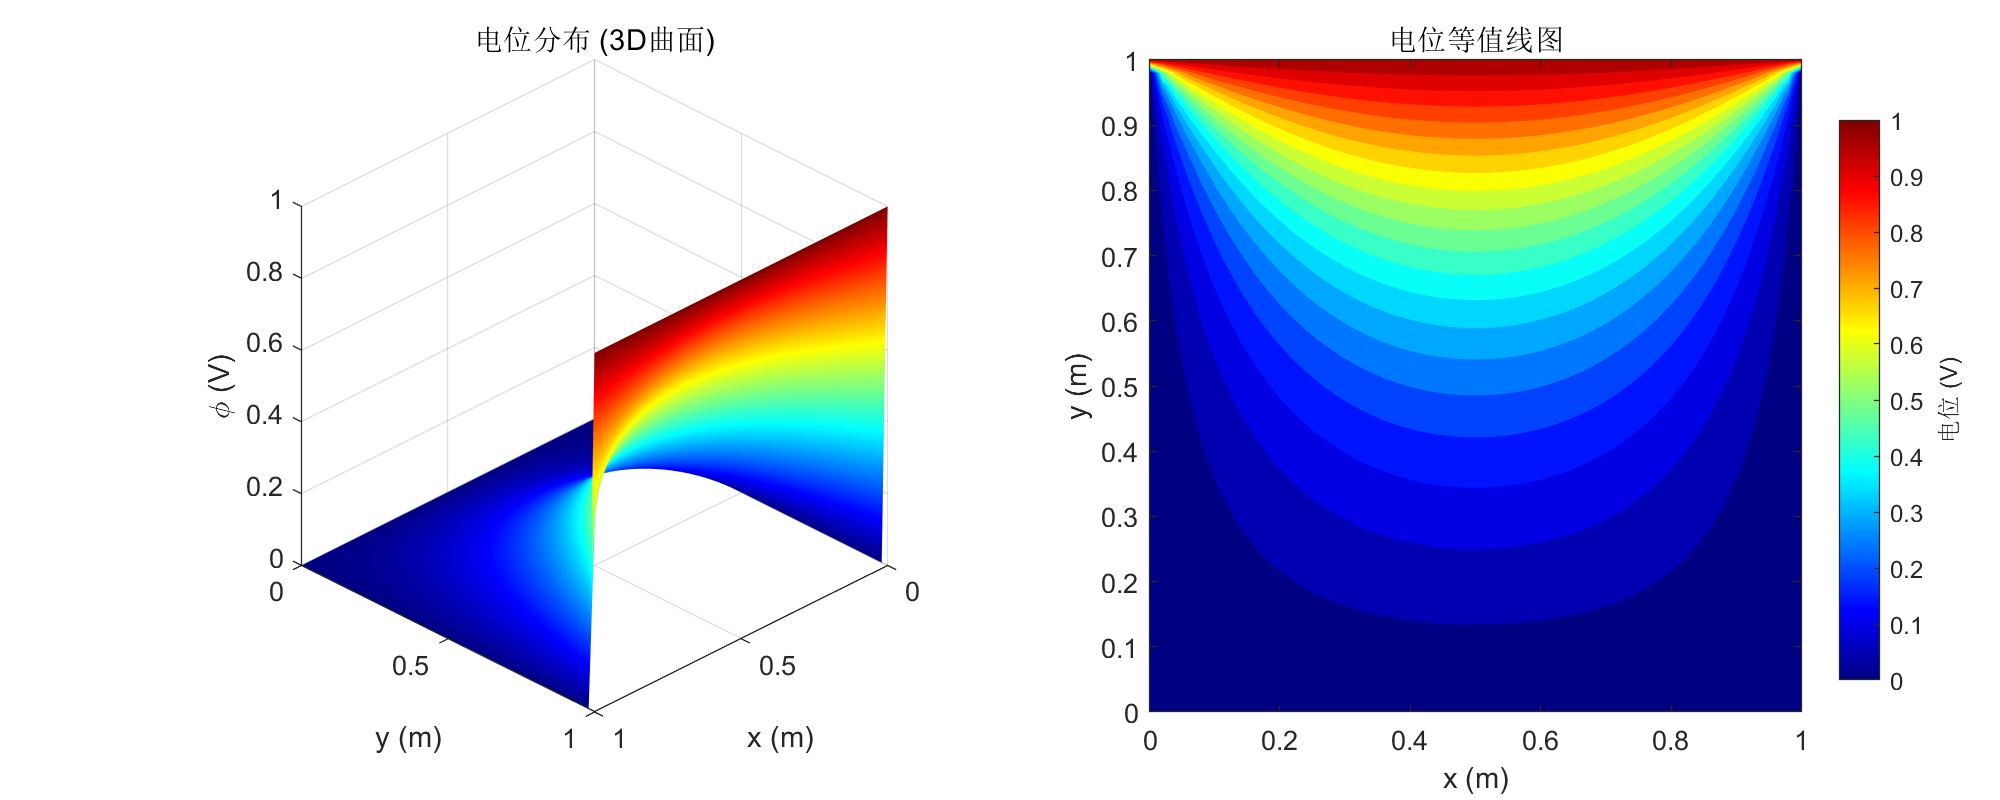
\includegraphics[width=0.9\linewidth]{fig1.png}
    \caption{上边界 1 V，其余接地。等值线呈水平状，电位沿 y 方向单调递减。}
\end{figure}

\begin{figure}[htbp]
    \centering
    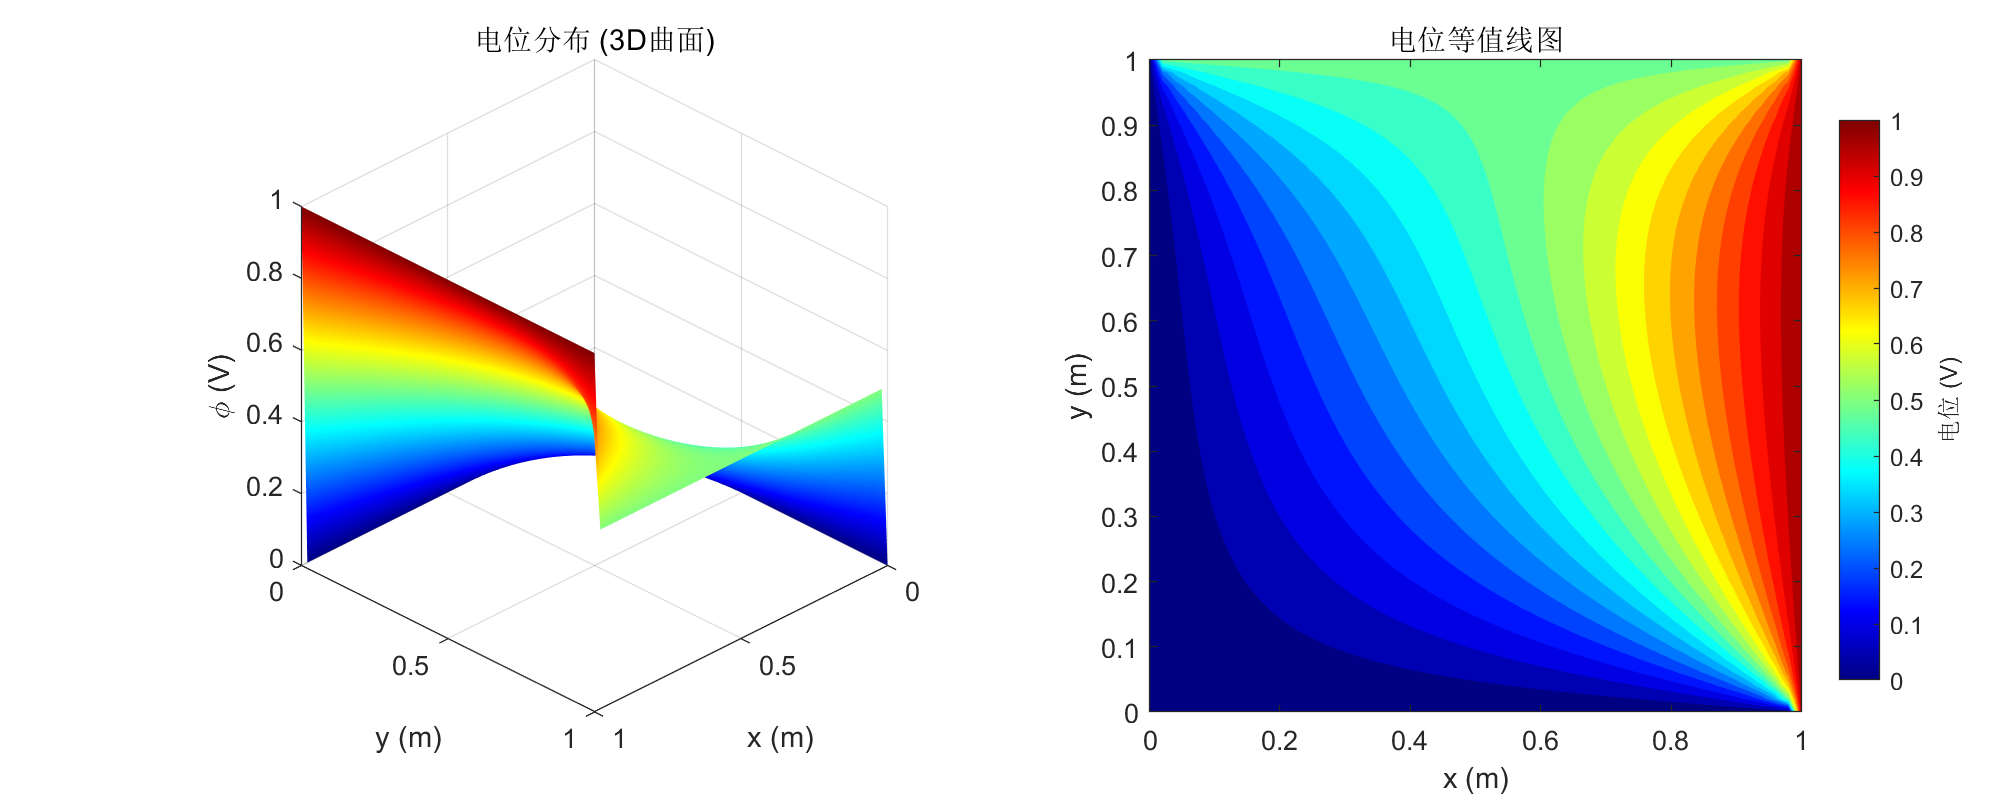
\includegraphics[width=0.9\linewidth]{fig2.png}
    \caption{上边界 0.5 V，右边界 1 V，其余接地。电位等值线向右上角集中，呈现非对称分布。}
\end{figure}

\begin{figure}[htbp]
    \centering
    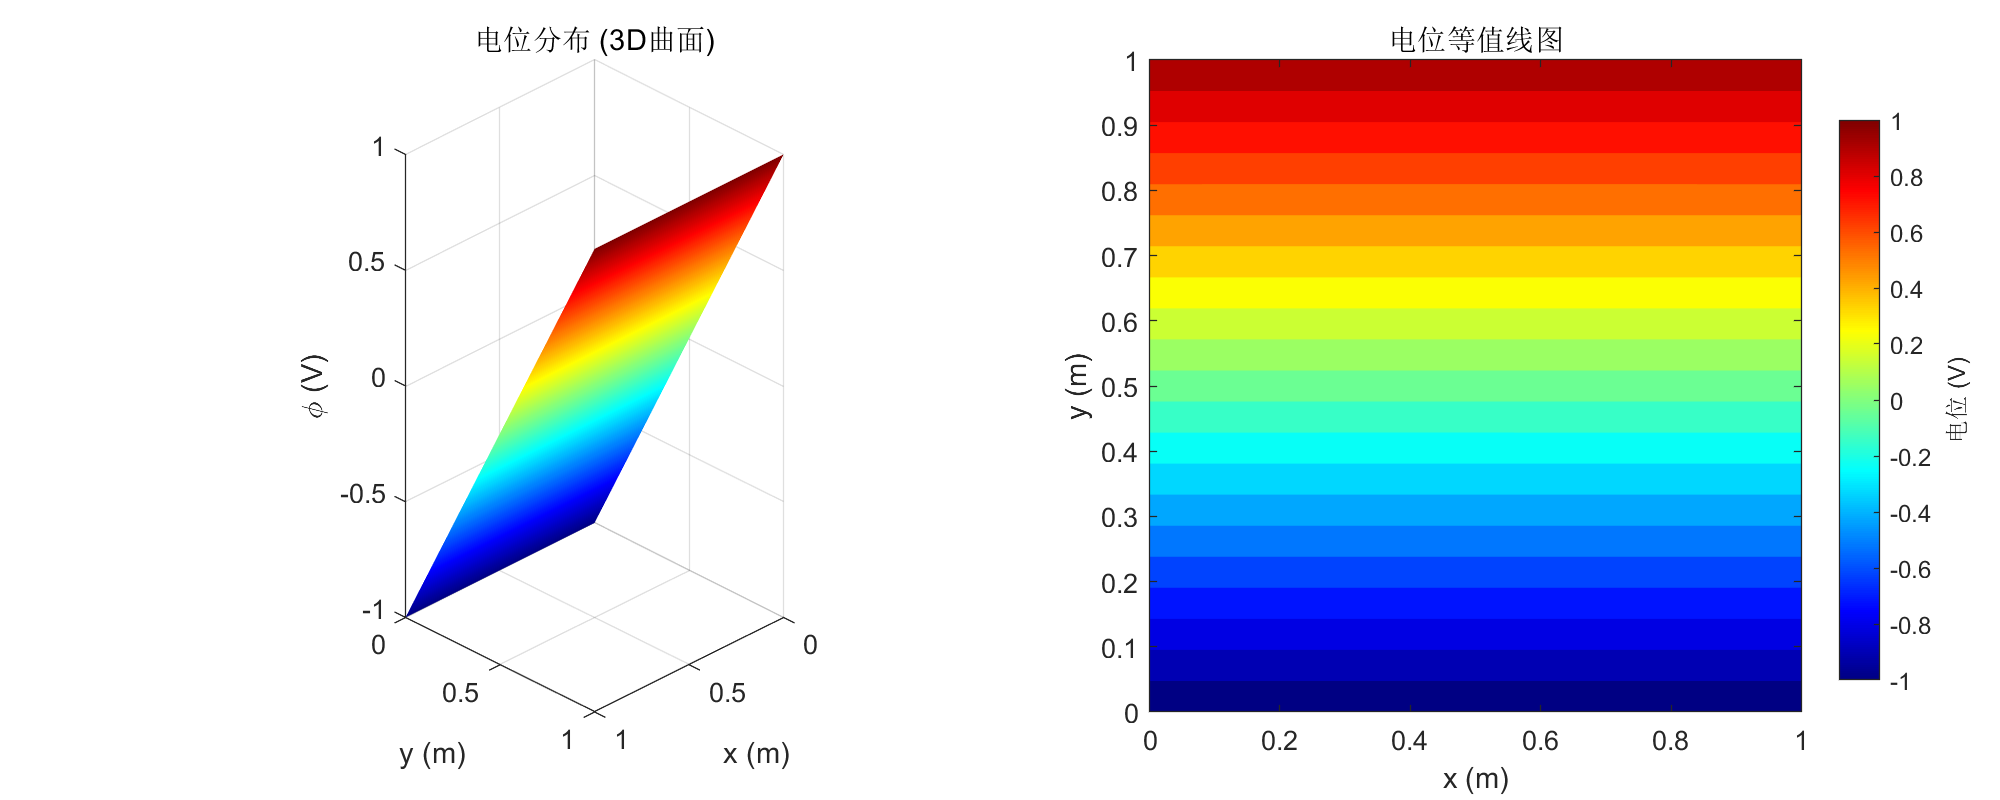
\includegraphics[width=0.9\linewidth]{fig3.png}
    \caption{上下边界 ±1 V，左右边界线性插值。电位沿 y 方向均匀变化，等值线为水平直线。}
\end{figure}

\begin{figure}[htbp]
    \centering
    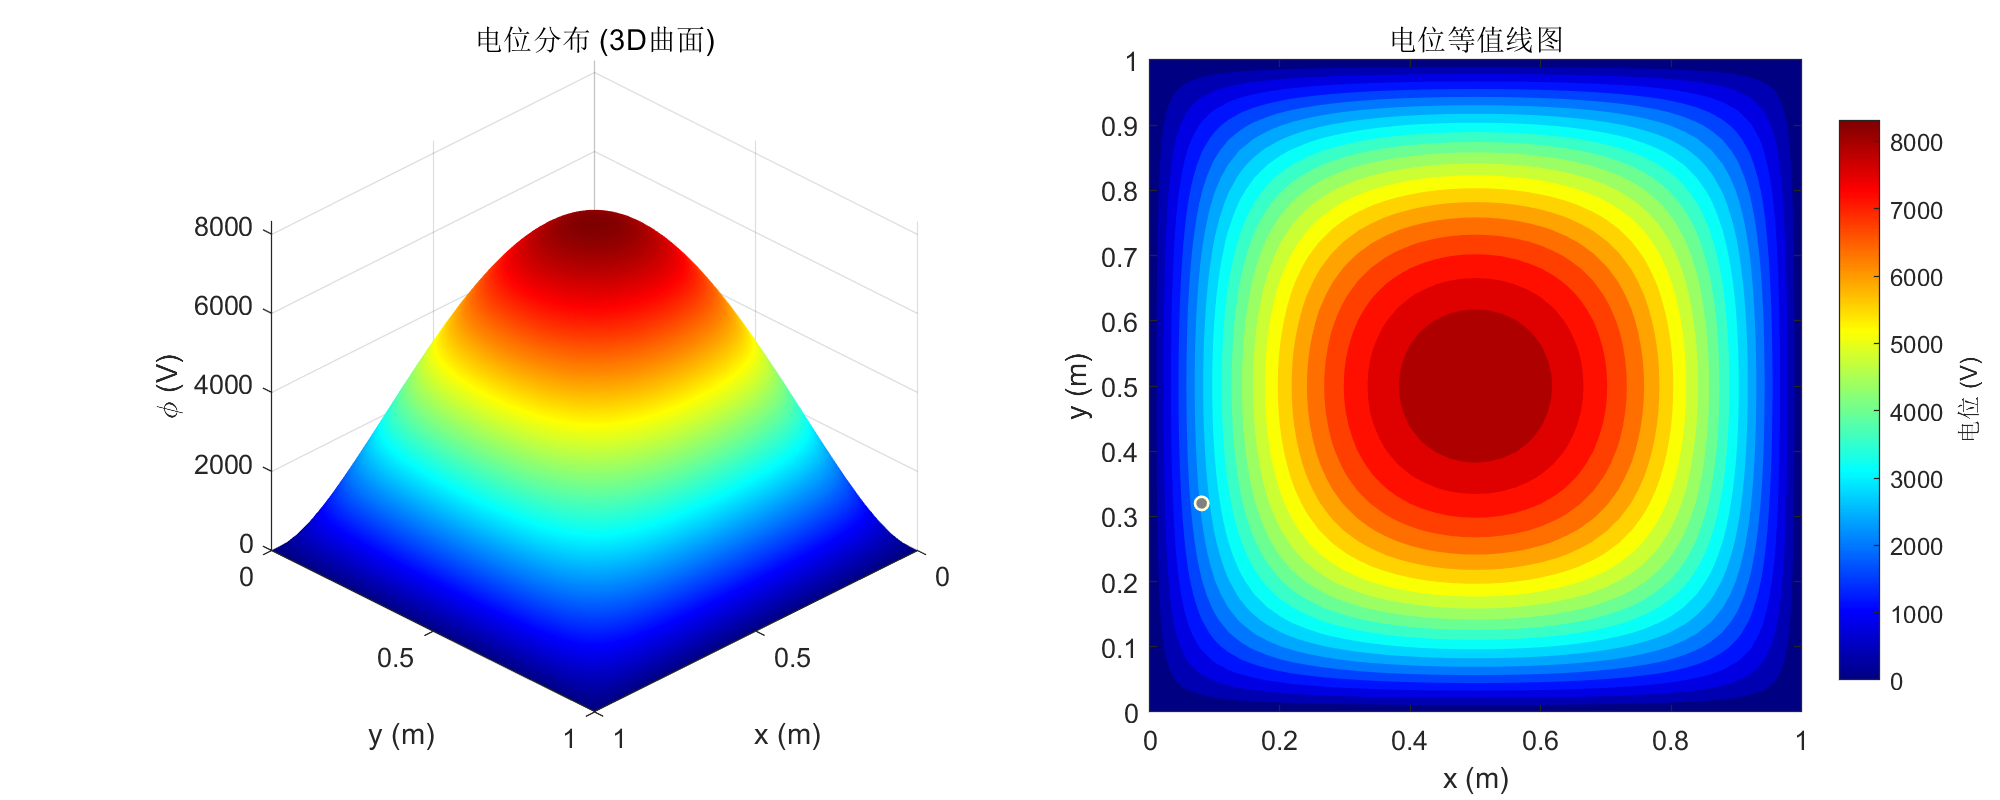
\includegraphics[width=0.9\linewidth]{fig4.png}
    \caption{四边接地，内部均匀体电荷 \(\rho=1\times10^{-6}\,\text{C/m}^3\)。电位呈中心对称分布，最大值位于区域中心。}
\end{figure}

\subsection{结果分析}

\begin{enumerate}
    \item \textbf{图1}：上边界为高电位（1 V），其余边界为低电位（0 V）。由于拉普拉斯方程具有调和性质，电位从顶部到底部逐渐平滑下降。
    \item \textbf{图2}：右上角存在两个高电位边界（上边界0.5 V，右边界1 V），导致该区域电位较高。内点电位介于0~1 V之间。
    \item \textbf{图3}：上下边界固定为±1 V，左右边界按线性插值设置。有限差分解与解析解（\(\phi=y\)）完全一致，等值线为严格的水平线。
    \item \textbf{图4}：四边接地，内部存在均匀面电荷。电位分布呈现类似抛物面（二维泊松方程）的形状，中心电位最高（约8800 V），向四周递减至0。
\end{enumerate}

\subsection{误差分析}
\begin{itemize}
    \item \textbf{截断误差}：采用中心差分近似二阶导数，截断误差为 \(O(h^2)\)。本实验 \(h=0.02\)，理论误差量级约 \(10^{-4}\)。
    \item \textbf{迭代误差}：收敛容差设为 \(10^{-6}\)，远小于截断误差，因此迭代误差可忽略。
    \item \textbf{边界条件处理}：对于 Dirichlet 边界，直接在边界节点赋值，无额外误差。
    \item \textbf{网格密度影响}：若增加网格数（如 \(101\times101\)），数值解将更接近真实解，但计算时间增加。本实验 \(51\times51\) 已能给出直观且足够准确的结果。
\end{itemize}

\section{个人总结与思考}

通过本次实验，我深入理解了有限差分法的基本原理及其在静电场数值求解中的应用。编写 Matlab 程序并利用 DeepSeek 辅助调试，提高了编程效率与代码可靠性。通过四种不同边界/源项的对比，直观地观察到边界条件与体电荷对电位分布的显著影响。

\begin{enumerate}
    \item \textbf{松弛因子 \(\omega\) 对收敛速度有何影响？}
    \par 当 \(1<\omega<2\) 时，适当增大 \(\omega\) 可加速收敛；若 \(\omega\) 接近 2 可能导致发散，\(\omega=1\) 时为高斯-赛德尔迭代。本实验采用 \(\omega=1.8\)，收敛步数约为高斯-赛德尔方法的 1/3，显著提高了效率。

    \item \textbf{若区域边界不是矩形，有限差分法如何处理？}
    \par 对于非矩形边界，可使用不规则网格或有限元法。若仍用有限差分法，需采用边界拟合坐标变换或对边界节点采用插值公式处理（如线性插值或镜像法），但实现较为复杂。

    \item \textbf{如何验证数值解的正确性？}
    \par 可通过以下方式验证：
    \begin{itemize}
        \item 与简单边界条件下的解析解对比。
        \item 检查数值解是否满足最大模原理（拉普拉斯方程的解在边界处取得最值）。
        \item 利用电荷守恒或能量积分进行辅助验证。
        \item 改变网格密度，观察解是否稳定收敛。
    \end{itemize}
\end{enumerate}

\section*{附录：MATLAB代码}

\begin{minted}{matlab}
% ====================================================
% 二维电位边值问题的有限差分法求解 (矩形域, 直角坐标)
% 方程: d^2φ/dx^2 + d^2φ/dy^2 = -ρ/ε
% ====================================================

clear; clc; close all;

% ---------- 物理与几何参数 ----------
Lx = 1.0;            % x方向长度
Ly = 1.0;            % y方向长度
eps0 = 8.854e-12;    % 真空介电常数 (若ρ=0可忽略)
rho = 0;             % 电荷密度 (C/m^3)，拉普拉斯方程设为0

% ---------- 网格参数 ----------
Nx = 51;             % x方向节点数 (含边界)
Ny = 51;             % y方向节点数 (含边界)
dx = Lx/(Nx-1);      % x方向步长
dy = Ly/(Ny-1);      % y方向步长

% ---------- 初始化 ----------
phi = zeros(Ny, Nx); % 电位矩阵 (行：y, 列：x)

% ---------- 边界条件 ----------
phi(1, :)  = 0.0;    % 下边界
phi(Ny, :) = 0.0;    % 上边界
phi(:, 1)  = 0.0;    % 左边界
phi(:, Nx) = 0.0;    % 右边界

% ---------- 源项（均匀体电荷，泊松方程） ----------
rho = 1e-6;          % 电荷密度 (C/m^3)
f = rho/eps0 * ones(Ny, Nx);

% ---------- 迭代参数 ----------
omega = 1.8;          % 松弛因子 (SOR)
tol = 1e-6;
maxIter = 10000;

% ---------- 迭代求解 (SOR) ----------
for iter = 1:maxIter
    phi_old = phi;
    maxErr = 0;

    for j = 2:Ny-1
        for i = 2:Nx-1
            if dx == dy
                h = dx;
                phi_new = 0.25 * (phi(j, i-1) + phi(j, i+1) 
                    + phi(j-1, i) + phi(j+1, i) + h^2 * f(j,i));
            else
                phi_new = ( (phi(j,i-1)+phi(j,i+1))/dx^2 
                    + (phi(j-1,i)+phi(j+1,i))/dy^2 + f(j,i) ) / (2/dx^2 + 2/dy^2);
            end
            phi(j, i) = (1 - omega) * phi(j, i) + omega * phi_new;
            err = abs(phi(j, i) - phi_old(j, i));
            if err > maxErr, maxErr = err; end
        end
    end

    if maxErr < tol
        fprintf('迭代收敛于第 %d 步, 最大误差 = %.2e\n', iter, maxErr);
        break;
    end
end
if iter == maxIter
    fprintf('达到最大迭代次数 %d, 最大误差 = %.2e\n', maxIter, maxErr);
end

% ---------- 后处理与绘图 ----------
x = linspace(0, Lx, Nx);
y = linspace(0, Ly, Ny);
[X, Y] = meshgrid(x, y);

% 确定统一的颜色范围 (由电位数据的最小值和最大值决定)
cmin = min(phi(:));
cmax = max(phi(:));

% 创建图形窗口
figure('Position', [100, 100, 1000, 400]);

% ---- 子图1：三维曲面图 ----
subplot(1, 2, 1);
surf(X, Y, phi);
colormap(jet);
clim([cmin, cmax]);
shading interp;
xlabel('x (m)'); ylabel('y (m)'); zlabel('\phi (V)');
title('电位分布 (3D曲面)');
view(135, 30);
axis tight;

% ---- 子图2：二维等值线填色图 ----
subplot(1, 2, 2);
contourf(X, Y, phi, 20, 'LineColor', 'none');
clim([cmin, cmax]);
xlabel('x (m)'); ylabel('y (m)');
title('电位等值线图');
axis equal tight;

% ---- 添加共用的颜色条 ----
% 在右侧创建一个颜色条，位置与两个子图匹配
hp = get(gcf, 'Position');
cbar = colorbar;
cbar.Label.String = '电位 (V)';
% 将颜色条放在右侧合适位置
cbar.Position = [0.92, 0.15, 0.02, 0.7];
subplot(1,2,1);
daspect([1, 1, 1e4]);   
\end{minted}

\end{document}